%!TEX root = paper.tex
%===================================================================%
% Optimization
%===================================================================%
Solving the optimization problem \eqref{eqn:costfx} is challenging since the problem size $p$ is large and the three terms {in the cost function} can each be \mbox{non-differentiable}.
To address these challenges, we now introduce a scalable optimization framework based on augmented Lagrangian (AL) methods.
In particular, we introduce a variable splitting scheme that converts the unconstrained optimization problem of the form \eqref{eqn:costfx} into an equivalent constrained optimization problem, which can be solved efficiently using the alternating direction method of multipliers (ADMM) algorithm \citep{Boyd:2011,Glowinski:1975, Gabay:1976}. 
We demonstrate that by augmenting the weight vector with zero entries at appropriate locations, the inner subproblems associated with ADMM can be solved efficiently in closed form.

%===================================================================%
\subsubsection{Alternating Direction Method of Multipliers}
The ADMM algorithm is a powerful algorithm for solving convex optimization problems having the separable structure \citep{Boyd:2011}
\begin{equation}
	\minimize{\xbar,\ybar}\,\fbar(\xbar) + \gbar(\ybar) \;\;\;\; 
	\text{subject to } \Abar\xbar+\Bbar\ybar=\bzero \;,
	\label{eqn:canonical,admm}
\end{equation}
where $\xbar\in\reals^\pbar$ and $\ybar\in\reals^\qbar$ are unknown primal variables, $\fbar:\reals^\pbar\to\reals\cup\{+\infty\}$ and $\gbar:\reals^\qbar\to\reals\cup\{+\infty\}$ are closed convex functions, and $\Abar\in\reals^{c\times \pbar}$ and $\Bbar\in\reals^{c\times \qbar}$ are matrices representing $c$ linear constraints.  
More specifically, the ADMM algorithm solves for the primal variables in \eqref{eqn:canonical,admm} through the following iterative procedure:
\begin{align}
	&\hspace{0.17\linewidth}\xbar\iterp\leftarrow\displaystyle\argmin{\xbar} \fbar(\xbar) + \frac{\rho}{2}\norm{\Abar\xbar + \Bbar\ybar\iter + \u\iter}^2 \label{eqn:admm,xbar,update}\\ 
	&\hspace{0.17\linewidth}\ybar\iterp\leftarrow\displaystyle\argmin{\ybar} \gbar(\ybar) + \frac{\rho}{2}\norm{\Abar\xbar\iterp + \Bbar\ybar + \u\iter}^2 \label{eqn:admm,ybar,update}\\ 
	&\hspace{0.17\linewidth}\u\iterp\leftarrow \u\iter+ \left(\Abar\xbar\iterp+\Bbar\ybar\iterp\right)  \; , & \label{eqn:admm,dual,update}
\end{align}
where superscript $t$ denotes the iteration count and $\u\in\reals^c$ denotes the (scaled) dual variable.

The convergence of the ADMM algorithm has been established in Theorem $1$ of \cite{Mota:2011}, which states that if matrices \Abar and \Bbar are full column-rank and the problem \eqref{eqn:canonical,admm} is solvable (\ie, it has an optimal objective value), the ADMM iterations \eqref{eqn:admm,xbar,update} - \eqref{eqn:admm,dual,update} converges to the optimal solution.
While the AL parameter $\rho>0$ does not affect the convergence property of ADMM, it can impact its convergence speed.
We use the value $\rho=1$ in all of our implementations.

%===================================================================%
\subsubsection{Variable splitting and data augmentation}
\label{subsec:var,split}
The original formulation of our problem \eqref{eqn:costfx} does not have the structure of \eqref{eqn:canonical,admm}.
However, we can convert the unconstrained optimization problem \eqref{eqn:costfx} into an equivalent constrained optimization problem \eqref{eqn:canonical,admm} by introducing auxiliary constraint variables, a method known as \emph{variable splitting} \citep{Afonso:2010}.  
While there are several different ways to introduce the constraint variables, the heart of the strategy is to select a splitting scheme that decouples the problem into more manageable subproblems.
For example, one particular splitting strategy we can adopt for problem \eqref{eqn:costfx} is
\begin{equation}
	\begin{array}{c}
		\dstyle\minimize{\substack{\w,\va \\ \vb,\vc,\vd}} 
			\frac{1}{n}\Loss(\va)+\lambda\norm{\vb}_1+\frac{\gamma}{q}\norm{\vc}^q_q \; \; 
			\vspace{0.01\linewidth}\\
		\text{ subject to }  \YXw =\va, \; \w=\vb, \; \C\vd=\vc, \;  \w=\vd \;, 
	\end{array}
	\label{eqn:splitting1}
\end{equation}
where $\va,\vb,\vc,\vd$ are the constraint variables.
It is easy to see that problems \eqref{eqn:costfx} and \eqref{eqn:splitting1} are equivalent, and the correspondence with the ADMM formulation \eqref{eqn:canonical,admm} is as follows:
\begin{equation}
	\begin{array}{c}
		\fbar(\xbar)=\dstyle\frac{\gamma}{q}\norm{\vc}^q_q , \;\;\;
		\gbar(\ybar)=\dstyle\frac{1}{n}\Loss(\va) + \lambda\norm{\vb}_1  
		\vspace{0.02\linewidth} \\
		\Abar = 	\ba{cc} 	\Y\X	& \bzero \\ \I	& \bzero \\ \bzero 	& \I \\ \I & \bzero \ea 	, \;
		\xbar = \bmat \w \\ \vc \emat, 
		\Bbar = 	\ba{rrr} 	-\I 	& \bzero	& \bzero \\ \bzero & -\I & \bzero  \\ 
						 \bzero & \bzero & -\C \\ \bzero & \bzero & -\I \ea,
		\ybar = \bmat \va \\ \vb \\ \vd \emat 	.
	\end{array}
	\label{eqn:admm,objective1}
\end{equation}
However, there is an issue with this splitting strategy: one of the resulting subproblems from the ADMM algorithm requires us to invert a matrix involving the Laplacian matrix $\C^T\C\in\reals^{p\times p}$, which is prohibitively large.
Although this matrix is sparse, it has a distorted structure due to the irregularities in the coordinates of \x.
These irregularities arise from two reasons:
(1) the nodes defining the functional connectome \x are placed only on the brain, not the entire rectangular field of view (FOV), and
(2) \x lacks a complete $6$-D representation since it only contains the lower-triangular part of the cross-correlation matrix.
Fig.~\ref{fig:lap,noncirc} displays the Laplacian matrix that results from the $347$-node functional connectome defined in Section~\ref{subsec:FC,def}, and the distorted structure is clearly visible.

To address this issue, we introduce an \emph{augmentation matrix} $\A\in\reals^{\ptil\times p}$, whose rows are either the zero vector or an element from the trivial basis $\braces{\bmath{e}_j \; |\; j\in[p]}$, and has the property $\A^T\A=\I_p$.
Furthermore, we define the \emph{augmented weight vector} $\wtil:=\A\w$, where \A rectifies the irregularities in the coordinates of \w (and \x) by padding extra zero entries, accommodating for:
(1) the nodes that were not placed in the FOV (\ie, the regions outside the brain), and
(2) the diagonal and upper-triangular part of the cross-correlation matrix, which were disposed due to redundancy; further details regarding this augmentation scheme is reported in \ref{appendix:data,aug}.
As a result, we now have a new differencing matrix $\Ctil\in\reals^{\tilde{e}\times\ptil}$ corresponding to $\wtil\in\reals^\ptil$, whose Laplacian matrix $\Ctil^T\Ctil\in\reals^{\ptil\times\ptil}$ has a systematic structure, as shown in Fig.~\ref{fig:lap,circ}.
In fact, this matrix has a special structure known as \emph{block-circulant with circulant-blocks} (BCCB), which is critical since the matrix inversion involving $\Ctil^T\Ctil$ can be computed efficiently in closed form using the fast Fourier transform (FFT) (the utility of this property will be elaborated more in Section~\ref{subsec:admm,steps}).  
It is important to note that this BCCB structure in the Laplacian matrix arises from the grid structure introduced from the parcellation scheme we adopted for producing the functional connectome.

%********** Laplacian matrix figures ****************%
\renewcommand{\imwidth}  {0.38\linewidth}
\begin{figure}
	\centering
	\begin{subfigure}[t]{\imwidth}
		 \centering
		 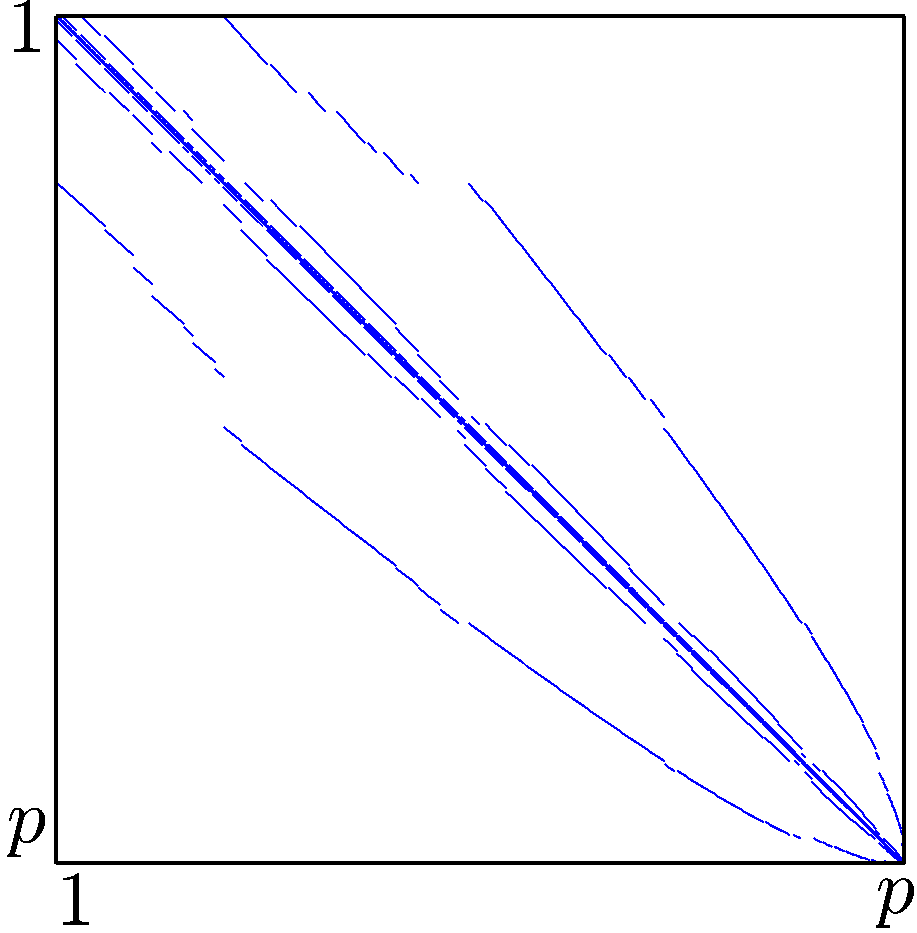
\includegraphics[height=.7\linewidth]{\fig/laplacemat_noncirc.pdf}
		 \caption{Laplacian matrix: $\C^T\C$}
		 \label{fig:lap,noncirc}
	\end{subfigure}
%	\hfill
	\hspace{0.05\linewidth}
	\begin{subfigure}[t]{\imwidth}
		 \centering
		 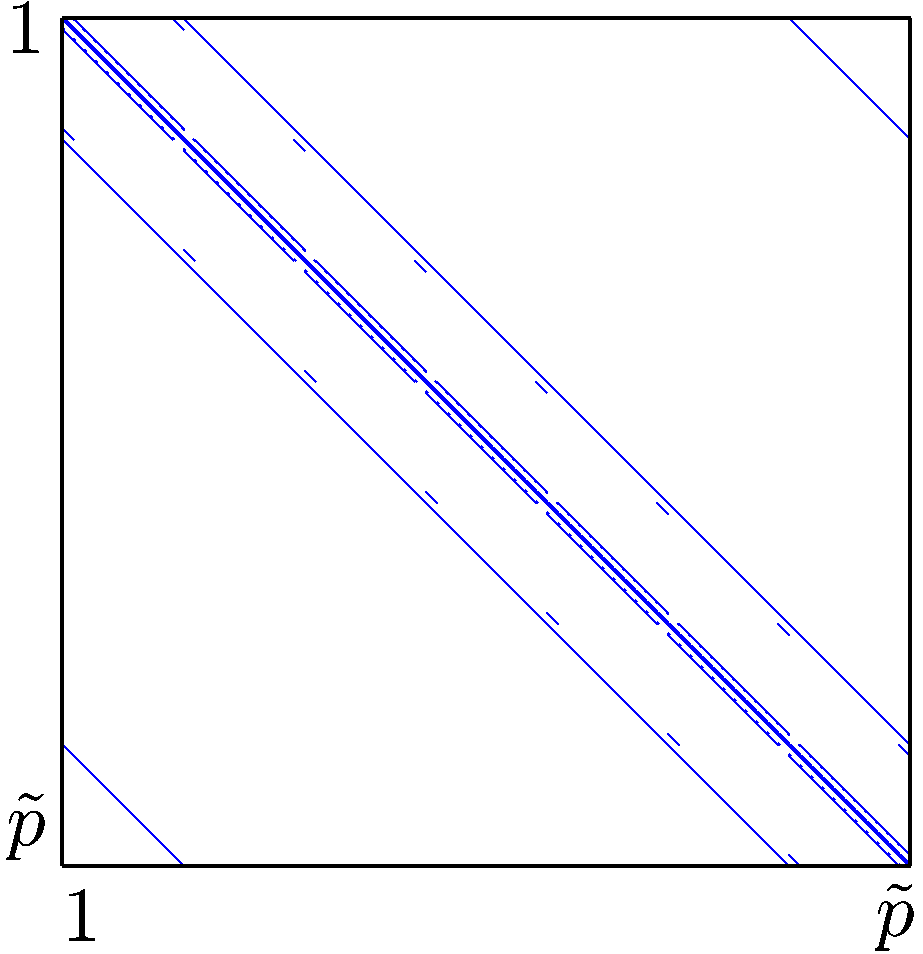
\includegraphics[height=.7\linewidth]{\fig/laplacemat_circ.pdf}
		 \caption{Augmented Laplacian matrix: $\Ctil^T\Ctil$}
		 \label{fig:lap,circ}
	\end{subfigure}

	\caption{Laplacian matrix corresponding to the original data $\C^T\C$ and the augmented data $\Ctil^T\Ctil$, where the rows and columns of these matrices represent the coordinates of the original and augmented functional connectome.  Note that the irregularities in the original Laplacian matrix are rectified by data augmentation.  The augmented Laplacian matrix has a special structure known as \emph{block-circulant with circulant-blocks} (BCCB), which has important computational advantages that will be exploited in this work.}
	 \label{fig:lap}
\end{figure}
%********************************************************%

Finally, by introducing a diagonal masking matrix $\B\in\{0,1\}^{\ptil\times\ptil}$, we have $\|\B\Ctil\wtil\|^q_q = \norm{\C\w}_q^q$ for $\q\in\{1,2\}$.  
Note that this masking strategy was adopted from the recent works of \cite{Allison:2013} and \cite{Matakos:2013}, and has the effect of removing artifacts that are introduced from the data augmentation procedure when computing the $\norm{\cdot}_q^q$-norm.
This allows us to write out the fused Lasso and GraphNet problem \eqref{eqn:costfx} in the following equivalent form:
\begin{equation}
	\argmin{\w\in\reals^p} \frac{1}{n}\Loss(\YXw) + \lambda\norm{\w}_1 + 
		\frac{\gamma}{q}\norm{\B\Ctil\A\w}^q_q  \; ,\; q\in\{1,2\}
	\nonumber
\end{equation}
Moreover, this can be converted into a constrained optimization problem
\begin{equation}
	\begin{array}{c}
		\dstyle\minimize{\substack{\w,\va \\ \vb,\vc,\vd}} 
			\frac{1}{n}\Loss(\va)+\lambda\norm{\vb}_1+\frac{\gamma}{q}\norm{\B\vc}^q_q \; \; 
			\vspace{0.01\linewidth}\\
		\text{ subject to }  \YXw =\va, \; \w=\vb, \; \Ctil\vd=\vc, \;  \A\w=\vd \;, 
	\end{array}
	\label{eqn:admm,splitting2}
\end{equation}
and the correspondence with the ADMM formulation \eqref{eqn:canonical,admm} now becomes:
\begin{equation}
	\begin{array}{c}
		\fbar(\xbar)=\dstyle\frac{\gamma}{q}\norm{\B\vc}^q_q , \;\;\;
		\gbar(\ybar)=\dstyle\frac{1}{n}\Loss(\va) + \lambda\norm{\vb}_1  
		\vspace{0.02\linewidth} \\
		\Abar = 	\ba{cc} 	\Y\X	& \bzero \\ \I	& \bzero \\ \bzero 	& \I \\ \A & \bzero \ea 	, \;
		\xbar = \bmat \w \\ \vc \emat 			, 
		\Bbar = 	\ba{rrr} 	-\I 	& \bzero	& \bzero \\ \bzero & -\I & \bzero  \\ 
						 \bzero & \bzero & -\Ctil \\ \bzero & \bzero & -\I \ea 		, 
		\ybar = \bmat \va \\ \vb \\ \vd \emat \;.
	\end{array}
	\label{eqn:admm,objective2}
\end{equation}
The dual variables corresponding to $\va,\vb,\vc,$ and $\vd$ are written in block form $\u=[\ua^T,\ub^T,\uc^T,\ud^T]^T$.
Note that functions \fbar and \gbar are convex, and matrices \Abar and \Bbar are full column-rank, so the convergence of the ADMM iterations \eqref{eqn:admm,xbar,update}-\eqref{eqn:admm,dual,update} is guaranteed (see Theorem~1 in \cite{Mota:2011}).

%===================================================================%
\subsubsection{ADMM: efficient closed-form updates}
\label{subsec:admm,steps}

With the variable splitting scheme \eqref{eqn:admm,splitting2} and ADMM formulation \eqref{eqn:admm,objective2}, the ADMM update for the primal variable $\xbar$ \eqref{eqn:admm,xbar,update} decomposes into subproblems
\begin{alignat}{1} 
	\w\iterp 	\leftarrow \argmin{\w}&
		 \Bigg\{\normsq{\Y\X\w-\left(\va\iter-\ua\iter\right)} 
		+ \normsq{\w-\left(\vb\iter-\ub\iter\right)} \nonumber \\
		  &+ \normsq{\A\w-\left(\vd\iter-\ud\iter\right)} \Bigg\} \label{eqn:w,update1} \\
	\vc\iterp \leftarrow \argmin{\vc}&
		\Bigg\{\frac{\gamma}{q}\norm{\B\vc}_q^q
		  +\frac{\rho}{2}\normsq{\vc-\left(\Ctil\vd\iter-\uc\iter\right)}\Bigg\}\;, \label{eqn:v3,update1}
\end{alignat}
whereas the updates for primal variable $\ybar$ \eqref{eqn:admm,ybar,update} are
\begin{alignat}{1} 
	\va\iterp \leftarrow \argmin{\va}
		& \left\{ \frac{1}{n}\Loss(\va) + \frac{\rho}{2}\normsq{\va-\left(\Y\X\w\iterp+\ua\iter\right)} \right\}
			\label{eqn:v1,update1}\\
	\vb\iterp \leftarrow \argmin{\vb} 
		& \left\{\lambda\norm{\vb}_1 + \frac{\rho}{2}\normsq{   \vb-\left(\w\iterp+\ub\iter\right)} 
			\label{eqn:v2,update1}\right\}\\
	\vd\iterp \leftarrow \argmin{\vd}
		& \bigg\{\normsq{\Ctil\vd-\left(\vc\iterp+\uc\iter\right)}
		 + \normsq{\vd-\left(\A\w\iterp+\ud\iter\right)}\bigg\} \;.  \label{eqn:v4,update1}
\end{alignat}
The update for the dual variable \u is a trivial matrix-vector \mbox{multiplication \eqref{eqn:admm,dual,update}} (see Algorithm~\ref{alg:admm} line $14$-$17$).

We now demonstrate that the minimization problems \eqref{eqn:w,update1}-\eqref{eqn:v4,update1} each admits an efficient, closed form solution.

\newcommand{\Bvarrho}{\bmath{\varrho}}
%--------------------------------------------------%
\paragraph{\w update}
The quadratic minimization problem \eqref{eqn:w,update1} has the following closed form solution:
\begin{align}
	\w\iterp \leftarrow \left(\X^T\X + 2\BI_p\right)\inv  
		\Big(&\X^T\Y^T [\va\iter-\ua\iter] 
		+[\vb\iter-\ub\iter]  
		 +\A^T[\vd\iter-\ud\iter] \Big) \,. \label{eqn:w,update2}
\end{align}
Note we used the fact that $\Y^T\Y=\I_n$ and $\A^T\A=\I_p$ to arrive at this expression.
Applying update \eqref{eqn:w,update2} brute force will require an inversion of a $(p\times p)$ matrix, but this can be converted into an $(n\times n)$ inversion problem by invoking the \emph{matrix inversion Lemma}
\begin{equation}
	\left( \X^T\X + 2\BI_p   \right)\inv = 
	\frac{1}{2}\I_p - \frac{1}{4}\X^T \big( \I_n + \frac{1}{2}\X\X^T \big)\inv\X \; .
	\label{eqn:inv,lemma}
\end{equation}
In the context of our work, $n$ denotes the number of scanned subjects, which is typically on the order of a few hundred.
The matrix $(\X^T\X + 2\BI_p)\inv$ can be stored in memory if $p$ is small, but the massive dimensionality of the functional connectome in our application dismisses this option.
Therefore, we instead precompute the $(p\times n)$ matrix $\BH:=\frac{1}{4}\X^T(\I_n+\frac{1}{2}\X\X^T)\inv$ in~\eqref{eqn:inv,lemma}, and let
\[\Bvarrho\iter:=\X^T\Y^T [\va\iter-\ua\iter] +[\vb\iter-\ub\iter] +\A^T[\vd\iter-\ud\iter]\;.\]
This way, the update \eqref{eqn:w,update2} can be implemented as follows:
\begin{equation}
	w\iterp \leftarrow(\X^T\X + 2\I_p)\inv\Bvarrho\iter=\frac{1}{2}\Bvarrho\iter - \BH\X\Bvarrho\iter\;,
	\label{eqn:inv,lemma2}
\end{equation}
which allows us to carry out the \w-update without having to store a $(p\times p)$ matrix in memory.

%--------------------------------------------------%
\paragraph{\va and \vb update}
The minimization problems \eqref{eqn:v1,update1} and \eqref{eqn:v2,update1} have the form of the (scaled) proximal operator $\prox_{\tau F}:\reals^p\to\reals^p$ \citep{Rockafellar:1998:book}, defined by 
\begin{equation}
	\prox_{\tau F}(\Bv)= \argmin{\Bu\in\reals^p}\tau F(\Bu)+\frac{1}{2}\norm{\Bv-\Bu}^2 ,\;\; \tau>0\;,
	\label{eqn:prox}
\end{equation}
where $F:\reals^p\to\reals\cup\{+\infty\}$ is a closed convex function.
Using standard subdifferential calculus rules \citep{Borwein:2006:book}, it is straightforward to show that a point $\u^*\in\reals^p$ solves the minimization in \eqref{eqn:prox} if and only if the condition 
\begin{equation}
	\bzero\in \partial F(\u^*)+(\u^*-\Bv)/\tau
	\label{eqn:prox,opt,cond}
\end{equation} 
holds.
Here, $\partial F(\u^*)$ denotes the subdifferential of function $F$ at $\u^*$, defined by 
\begin{equation}
	\partial F(\u^*):= \left\{ \Bz\in\reals^p :
		 F(\u^*) + \inprod{\Bz,\u-\u^*} \leq F(\u),\; \forall \u\in\reals^p
						\right\}     .
\nonumber
\end{equation}

In addition, both updates \eqref{eqn:v1,update1} and \eqref{eqn:v2,update1} are fully separable across their coordinates, decomposing into the following sets of elementwise scalar optimization problems:
\begin{alignat}{3} 
  \left[\va\iterp\right]_i \;\;\leftarrow \;\;&
  	\prox_{\frac{\loss}{n\rho}}\left(\big[ \Y\X\w\iterp + \ua\iter \big]_i\right) ,
  	& \;\;\;\;\;\; i\in[n] \label{eqn:v1,update2} \\
  \left[\vb\iterp\right]_j \;\;\leftarrow \;\;&
  	\prox_{\frac{\lambda}{\rho}\abs{\cdot}}\left(\big[ \w\iterp+\ub\iter \big]_j\right) ,
  	& j\in[p] &\;,\label{eqn:v2,update2} 
\end{alignat}
where $[\,\cdot\,]_i$ and $[\,\cdot\,]_j$ each index the $i$-th and $j$-th element of a vector in $\reals^n$ and $\reals^p$ respectively.
For some margin-based loss functions, their corresponding proximal operator \eqref{eqn:v1,update2} can be derived in closed form using the optimality condition~\eqref{eqn:prox,opt,cond}.
Fig.~\ref{fig:prox} plots a few commonly used margin-based losses and their corresponding proximal operators, and Table~\ref{table:prox} provides their closed form expressions.
The choice of the margin-based loss is application dependent, such as whether differentiability is desired or not.
The proximal operator of the \ellone-norm~\eqref{eqn:v2,update1} and the absolute loss function~\eqref{eqn:v2,update2} corresponds to the well known \emph{soft-threshold operator} \citep{Donoho:1995}
\begin{equation}
	\text{Soft}_\tau(t):=
		\begin{cases}
			t-\tau & \text{if } t > \tau \\
			0		& \text{if } \abs{t}\leq \tau \\
			t+\tau	& \text{if } t < -\tau
		\end{cases} \;\;.
	\label{eqn:soft,thresh}
\end{equation}
The absolute loss and the soft-threshold operator are also included in Fig.~\ref{fig:prox} and Table.~\ref{table:prox} for completeness.

% figure table of loss functions and prox functions in this work
%======================= Proximal operators =============================%
\afterpage{%    % defer execution until the next page break occurs anyway
\renewcommand{\imwidth}  {0.365\linewidth}
\renewcommand{\imwidthh}  {0.88\linewidth}
\begin{figure}[t!]
	\centering
	\begin{subfigure}[t]{\imwidth}
		 \centering
		 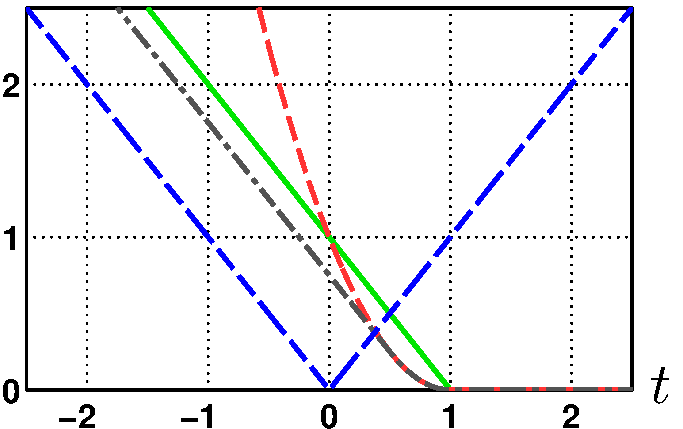
\includegraphics[width=\imwidthh]{\fig/prox_map_loss.pdf}
		 \caption{{Loss functions $\loss(t)$}}
		 \label{subfig:loss,fcn}
	\end{subfigure}
%	\hfill
	\begin{subfigure}[t]{0.225\linewidth}
		 \centering
		 \raisebox{0.17\linewidth}{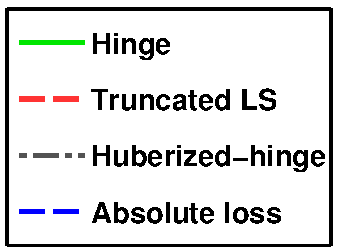
\includegraphics[width=\imwidthh]{\fig/prox_map_legend.pdf}}
	\end{subfigure}
%	\hfill
	\begin{subfigure}[t]{\imwidth}
		 \centering
		 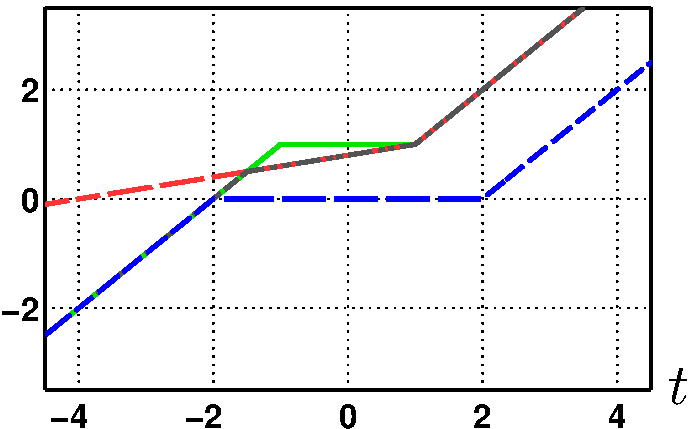
\includegraphics[width=\imwidthh]{\fig/prox_map_prox.pdf}
		 \caption{{Proximal operator $\prox_{\tau\loss}(t)$}}
		 \label{subfig:loss,prox}
	\end{subfigure}%
	\caption{Plots of scalar convex loss functions that are relevant in this work, along with their associated proximal operators. 
	  Table~\ref{table:prox} provides the closed form expression for these functions.  
	  Parameter values of $\tau=2$ and $\delta=0.5$ are used in the plot for the proximal operator and the huberized hinge-loss respectively.}
	\label{fig:prox}
\end{figure}
\begin{table}[h!]\small
	\centering
	\begin{tabular}{c|c|l}
		& \normalsize{$\loss(t)$} & \hspace{0.1\linewidth}\normalsize{$\prox_{\tau\loss}(t)$}\\
		\hline\hline  %<- requires the "booktabs" package
		 Hinge 			& $\max(0,1-t)$ 	& 
			 $\begin{cases}
				t 		& \text{if } t>1\\
				1 		& \text{if } 1-\tau\leq t \leq 1 \\
				t+\tau	& \text{if } t < 1-\tau
			 \end{cases}$\\ \hline
		 \begin{tabular}{c}Truncated\\ least squares\end{tabular}	
		 	& $\big\{\max(0,1-t)\big\}^2$	& 
		 	$\begin{cases}
		 		t			& \text{if } t>1 \\
		 		\dstyle\frac{t+2\tau}{1+2\tau}	& \text{if } t\leq 1 \\
		 	\end{cases}$\\ \hline
		  \begin{tabular}{c}Huberized\\ hinge \\ \citep{Wang:2008} \end{tabular}		& 
			 $\begin{cases}
				0 					&\text{if } t>1 \\
			 	\dstyle\frac{(1-t)^2}{2\delta} 	&\text{if } 1-\delta \leq t \leq 1 \\
			 	 1-t-\frac{\delta}{2}	&\text{if } t < 1-\delta
			 \end{cases}$
			 & 
			 $\begin{cases}
				t 		&\text{if } t>1 \\
			 	\dstyle\frac{t+\tau/\delta}{1+\tau/\delta} 	&\text{if } 1-\delta-\tau \leq t \leq 1 \\
			 	t+\tau	&\text{if } t < 1-\delta-\tau
			 \end{cases}$ \\ \hline
		 \begin{tabular}{c}Absolute \\ loss\end{tabular}	
		 	& \begin{tabular}{c}
		 		$\abs{t}$\\ (from \ellone-regularization)
		 	  \end{tabular}	
		 	  & 
			 $\text{Soft}_\tau(t):=
			 \begin{cases}
			 	t-\tau & \text{if } t > \tau \\
			 	0		& \text{if } \abs{t}\leq \tau \\
			 	t+\tau	& \text{if } t < -\tau
			 \end{cases}$ \\
		\hline
	\end{tabular}
	\caption{Examples of scalar convex loss functions that are relevant for this work, along with their corresponding proximal operators in closed form.}
	\label{table:prox}
\end{table}
} % end of argument of `\afterpage` command
%=========================================================================%

%--------------------------------------------------%
\paragraph{\vc update}
The solution to the minimization problem \eqref{eqn:v3,update1} depends on the choice of $q\in\{1,2\}$, where $q=1$ recovers fused Lasso and $q=2$ recovers GraphNet.

In the fused Lasso case $q=1$, since the masking matrix $\B\in\{0,1\}^{\ptil\times\ptil}$ is diagonal, the update~\eqref{eqn:v3,update1} is fully separable.
Letting $\Bzeta\iter:=\Ctil\vd\iter-\uc\iter$, the minimization problem decouples into a set of scalar minimization problems of the form:
\begin{equation}
	\argmin{v_k\in\reals}\left\{ \gamma\; b_k\abs{v_k} + 
			\frac{\rho}{2} \left(v_k-\zeta_k\iter \right)^2  
		\right\} \;,\;\;\;\; k\in[\ptil]
	\label{eqn:v3,scalar}
\end{equation}
where $b_k$ is the $k$-th diagonal entry of \B and $\zeta_k\iter$ is the $k$-th entry of \sloppy{${\Bzeta\iter\in\reals^\ptil}$}.
On one hand, when $b_k=0$, the minimizer for problem~\eqref{eqn:v3,scalar} returns the trivial solution $\zeta_k\iter$.
On the other hand, when $b_k=1$, the minimizer will once again have the form of the proximal operator~\eqref{eqn:prox} corresponding to the absolute loss function $\abs{\cdot}$, recovering the soft-threshold operator~\eqref{eqn:soft,thresh}.
To summarize, when $q=1$, the update for \vc \eqref{eqn:v3,update1} can be done efficiently by conducting the following elementwise update for each $k\in[\ptil]$:
\begin{equation}
	\left[\vc\iterp\right]_k \;\leftarrow
	\begin{cases}
		\soft_{\gamma/\rho}\left(\left[\Ctil\left(\vd\iter-\uc\iter\right)\right]_k\right) & \text{if } \B_{k,k}=1 \\
		\left[\Ctil\left(\vd\iter-\uc\iter\right)\right]_k & \text{if } \B_{k,k}=0
	\end{cases}	
	\label{eqn:v3,update,flasso}
\end{equation}
where $\left[\cdot\right]_k$ indexes the $k$-th element of a vector in $\reals^\ptil$.

In the GraphNet case $q=2$, update \eqref{eqn:v3,update1} is a quadratic optimization problem with the closed form solution
\begin{equation}
	\vc\iterp \leftarrow \rho\big(\gamma\B+\rho\I_\ptil)\inv\Ctil(\vd\iter-\uc\iter) \;,
	\label{eqn:v3,update,gnet}
\end{equation}
which is trivial to compute since the matrix $(\gamma\B+\rho\I_\ptil)$ is diagonal.

%===================================================================%
\paragraph{\vd update}

The closed form solution to the quadratic optimization problem \eqref{eqn:v4,update1} is 
\begin{equation}
	\vd\iterp \leftarrow \left(\Ctil^T\Ctil + \I_\ptil\right)\inv
		\left(\Ctil^T[\vc\iter+\uc\iter]+\A\w\iterp+\ud\iter\right) \;.
	\label{eqn:v4,update2}
\end{equation}
To suppress notations, let us define $\Q\in\reals^{\ptil\times\ptil}$ and $\b\in\reals^\ptil$, where
$\Q:=\Ctil^T\Ctil + \I_\ptil$
and 
\[\b:=\Ctil^T[\vc\iter+\uc\iter]+\A\w\iterp+\ud\iter .\]
As stated earlier, the Laplacian matrix $\Ctil^T\Ctil$ is block-circulant with circulant-blocks (BCCB), and consequently, the matrix \Q is BCCB as well.  
It is well known that a BCCB matrix can be diagonalized as \citep{Davis:1979:book}
	\[\Q=\U^H\BLambda\U,\]
where $\U\in\reals^{\ptil\times\ptil}$ is the ($6$-D) DFT matrix and $\BLambda\in\reals^{\ptil\times\ptil}$ is a diagonal matrix containing the ($6$-D) DFT coefficients of the first column of \Q .
As a result, the update \eqref{eqn:v4,update2} can be carried out efficiently using the (6-D) FFT 
\begin{equation}
 	\Q\inv\b = 
 		\left(\U^H \BLambda\inv \U\right)\b = 
 		\mathrm{ifft}\Big(	\mathrm{fft}(\b)\odiv\Bphi \Big) \;,
 	\label{eqn:v4,fft}
\end{equation}
where $\text{fft}$ and $\text{ifft}$ denote the ($6$-D) FFT and inverse-FFT operation\footnote{These multidimensional FFT and inverse FFT operations are implemented using \texttt{fftn} and \texttt{iffn} functions in MATLAB.}, \Bphi is a vector containing the diagonal entries of \BLambda, and $\odiv$ indicates elementwise division 
(more precisely, vectors \b and \Bphi are reshaped into $6$-D arrays prior to the $6$-D FFT and inverse-FFT operations, and the result of these operations is re-vectorized).

AL-based optimization methods that involve this kind of FFT-based inversion have been applied in image processing \citep{Afonso:2010,Allison:2013, Matakos:2013}.
Problems such as image denoising, reconstruction, and restoration are typically cast as a regularized ERM problem involving the squared loss function.
The data augmentation scheme we propose allows us to apply this FFT-based technique with $6$-D functional connectomes in the context of binary classification with margin-based loss functions. 

Finally, note that the ADMM algorithm was also used to solve the fused Lasso regularized SVM problem in \citep{Gui-Bo-Ye:2011} under a different variable splitting setup.
However, their application focuses on $1$-D data such as mass spectrometry and array CGH.
Consequently, the Laplacian matrix corresponding to their feature vector is tridiagonal with no irregularities present.
Furthermore, the variable splitting scheme they propose requires an iterative algorithm to be used for one of the ADMM subproblems.
In contrast, the variable splitting scheme and the data augmentation strategy we propose allow the ADMM subproblems to be decoupled in a way that all the updates can be carried out efficiently and non-iteratively in closed form.

%--------------------------------------------------%
\paragraph{Summary: the final algorithm and termination criteria}
Algorithm~\ref{alg:admm} outlines the complete ADMM algorithm for solving both the fused Lasso and GraphNet regularized ERM problem \eqref{eqn:costfx}, and is guaranteed to converge.
In our implementations, all the variables were initialized at zero.
The algorithm is terminated when the relative difference between two successive iterates falls below a user-specified threshold:
\begin{equation}
	\frac{\norm{\w\iterp - \w\iter}}
		{\norm{\w\iter}}
	\leq \varepsADMM \;.
	\label{eqn:admm,termin}
\end{equation}

%****************** ADMM Algorithm ************************%
\newcommand{\indentAlg}{\hspace{0.05\linewidth}}
\begin{algorithm}[t!]
\caption{ADMM for solving fused Lasso $(q=1)$ or GraphNet $(q=2)$}
\label{alg:admm}
\begin{algorithmic}[1]
\begin{spacing}{1.2} 
\State Initialize primal variables $\w,\va,\vb,\vc,\vd$
\State Initialize dual variables $\ua,\ub,\uc,\ud$
\State Set $t=0$, assign $\lambda\geq 0,\, \gamma\geq 0$
\State Precompute $\BH:=\frac{1}{4}\X^T(\I_n+\frac{1}{2}\X\X^T)\inv$
\Repeat
	\State \xbar-update \eqref{eqn:admm,xbar,update}
		\State\indentAlg  $\w\iterp\leftarrow \left(\X^T\X + 2\BI_p\right)\inv  
		\big(\X^T\Y^T [\va\iter-\ua\iter] 
		+[\vb\iter-\ub\iter]  
		 +\A^T[\vd\iter-\ud\iter] \big)$\Statex\Comment{apply update \eqref{eqn:inv,lemma2}}
		\State\indentAlg $\vc\iterp \leftarrow 
			\begin{cases} 
				\text{solve using \eqref{eqn:v3,update,flasso}} & \text{if } q=1 \text{ (fused Lasso)}\\
				\text{solve using \eqref{eqn:v3,update,gnet}}   & \text{if } q=2 \text{ (GraphNet)}
			\end{cases}$
	\State \ybar-update \eqref{eqn:admm,ybar,update}
		\State\indentAlg $\va\iterp \leftarrow \prox_{\frac{\Loss}{n\rho}}\left(\Y\X\w\iterp+\ua\iter\right)$
			 \Comment{apply \eqref{eqn:v1,update2} elementwise}
		\State\indentAlg $\vb\iterp \leftarrow 
			\soft_{\lambda/\rho}\left(\w\iterp+\ub\iter\right)$
			\Comment{apply \eqref{eqn:v2,update2} elementwise}
		\State\indentAlg {\normalsize $\vd\iterp \leftarrow 
			\left(\Ctil^T\Ctil + \I_\ptil\right)\inv
			\left(\Ctil^T[\vc\iterp+\uc\iter]+\A\w\iterp+\ud\iter\right)$ \Statex\Comment{solve using FFT approach \eqref{eqn:v4,fft}}}
	\State \u-update \eqref{eqn:admm,dual,update}	
		\State\indentAlg $\ua\iterp \leftarrow \ua\iter + \Y\X\w\iterp-\va\iterp$
		\State\indentAlg $\ub\iterp \leftarrow \ub\iter + \w\iterp - \vb\iterp$
		\State\indentAlg $\uc\iterp \leftarrow \uc\iter + \vc\iterp - \Ctil\vd\iterp$
		\State\indentAlg $\ud\iterp \leftarrow \ud\iter + \A\w\iterp - \vd\iterp$
	\State $t\leftarrow t+1$
\Until{stopping criterion is met}
\end{spacing}
\end{algorithmic}
\end{algorithm}
%********************************************************%
